% Created 2022-06-01 Wed 11:29
% Intended LaTeX compiler: xelatex
\documentclass[11pt]{article}
\usepackage{graphicx}
\usepackage{longtable}
\usepackage{wrapfig}
\usepackage{rotating}
\usepackage[normalem]{ulem}
\usepackage{amsmath}
\usepackage{amssymb}
\usepackage{capt-of}
\usepackage{hyperref}
\usepackage{subcaption}
\usepackage{color}
\usepackage{listings}
\usepackage[newfloat]{minted}
\usepackage[utf8]{inputenc}
\usepackage[table,xcdraw]{xcolor}
\usepackage{paralist}
\usepackage{datetime2}
\usepackage{graphicx}
\usepackage{lscape}
\usepackage{longtable}
\usepackage{hyperref}
\usepackage[a4paper, left=3cm, right=3cm, top=2cm]{geometry}
\usepackage{fancyhdr}
\usepackage{listings}
\usepackage{textcomp}
\usepackage{enumitem}
\usepackage{algorithm}
\usepackage{algpseudocode}
\usepackage{subcaption}
\setlist{noitemsep}
\setlength{\columnseprule}{0.2pt}
\definecolor{mygreen}{rgb}{0,0.6,0}
\definecolor{mygray}{rgb}{0.5,0.5,0.5}
\definecolor{mymauve}{rgb}{0.58,0,0.82}
\lstset{ backgroundcolor=\color{white}, basicstyle=\footnotesize, breaklines=true, captionpos=b, commentstyle=\color{mygreen}, escapeinside={\%*}{*)},keywordstyle=\color{blue}, stringstyle=\color{mymauve},}
\author{Olivier Lischer}
\date{\today}
\title{Design Patterns - Summary}
\hypersetup{
 pdfauthor={Olivier Lischer},
 pdftitle={Design Patterns - Summary},
 pdfkeywords={},
 pdfsubject={},
 pdfcreator={Emacs 27.2 (Org mode 9.5.3)}, 
 pdflang={English}}
\begin{document}

\pagestyle{fancy}
\fancyhf{}
\fancyhead[R]{SEP2-FS}
\fancyhead[L]{Design Patterns - Summary}
\fancyfoot[CE,CO]{\leftmark}
\fancyfoot[R]{\thepage}
\fancyfoot[L]{Olivier Lischer}

\begin{titlepage}
  \begin{center}
    {\Huge Design Patterns - Summary} \\
    \vspace{8 cm}

    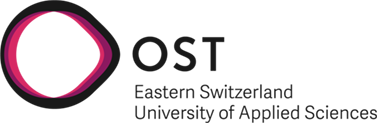
\includegraphics[height=4cm]{./img/ost-logo.png}

    \vspace{4 cm}
    Semester: Spring 2022
    \vspace{1 cm}

    Version: 0.1.0 \\
    Date: \DTMnow \\
    \vspace{3 cm}
    School of Computer Science\\
    OST Eastern Switzerland University of Applied Sciences
  \end{center}
\end{titlepage}
\newpage
\tableofcontents
\newpage


\section{Introduction}
\label{sec:org35b45ae}
\subsection{The design patterns}
\label{sec:orgfb8174d}

Class Design Patterns deal with the relationships between classes and their subclasses.
The Object Design Patterns with the object relationships which can be changed at runtime.

\begin{figure}[htbp]
\centering
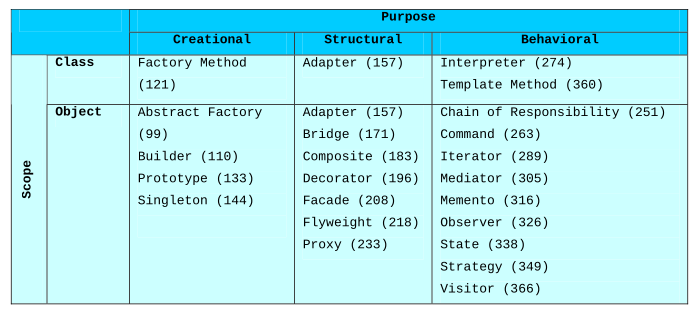
\includegraphics[width=0.6\textwidth]{img/design_pattern_space.png}
\caption{\label{fig:design-pattern-space}Design pattern space}
\end{figure}


\section{Design Patterns}
\label{sec:org0736d20}
\subsection{Creational Patterns}
\label{sec:orgf4a1e2c}
\subsubsection{Abstract Factory}
\label{sec:orgc2dcdc1}
The Abstract Factory provides an interface for creating families of related or dependent objects without specifying their concrete class.
It is a good choice, when you want to create big class hierarchy from a factory.
In general the Simple Factory is more common today.


Motivation:
\begin{itemize}
\item You want to create concrete objects without knowing which concrete type you get.
\item You are only interested in the interface.
\end{itemize}


\begin{figure}[htbp]
\centering
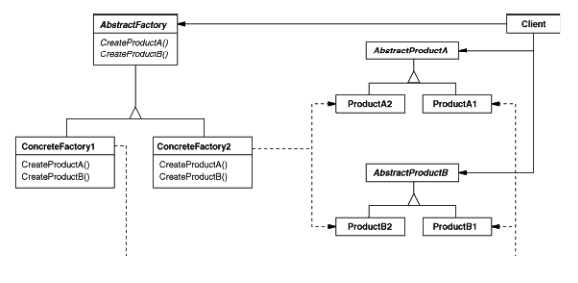
\includegraphics[width=0.6\textwidth]{img/abstract_factory.png}
\caption{\label{fig:abstract-factory-uml}Abstract Factory Class Diagram}
\end{figure}

\textbf{Important Notes:}
The Factory must be created at the very beginning of the application.
After creation only this factory must be used to create objects.
Otherwise, the benefit of the factory are gone.

\subsubsection{Builder}
\label{sec:org6e88d71}
The Builder Pattern separates the construction of a complex class from its representation.
Thereby you can hide the creation of complex objects behind functions.


\begin{figure}[htbp]
\centering
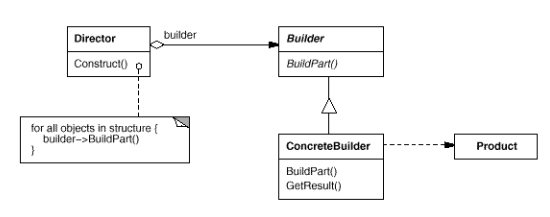
\includegraphics[width=0.6\textwidth]{img/builder.png}
\caption{\label{fig:builder-class-diagram}Builder Class Diagram}
\end{figure}
\subsubsection{Factory Method}
\label{sec:orgdd5dc83}
The Factory Method is used to create an object, but the subclass decides which class is instantiated.
With this pattern you can create concrete creators which can decide which concrete product should be created.
The user of the creator only has to use the interface.


\begin{figure}[htbp]
\centering
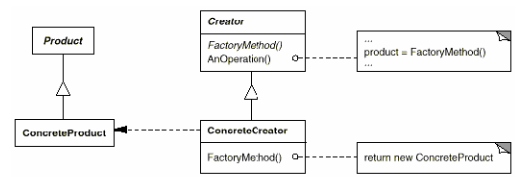
\includegraphics[width=0.6\textwidth]{img/factory_method.png}
\caption{\label{fig:factory-method-class-diagram}Factory Method Class Diagram}
\end{figure}

\subsubsection{Prototype}
\label{sec:org09c764f}
The prototype pattern is something similar for objects like the factory method is for classes.
Using the prototype pattern you create copies from concrete objects.
This is achieved by cloning the prototype.


\textbf{Important Notes:}
The crucial part of this pattern is the \texttt{Clone()} function.
During the implementation you have to decide if you want to do a deep copy or a shallow copy.


\begin{figure}[htbp]
\centering
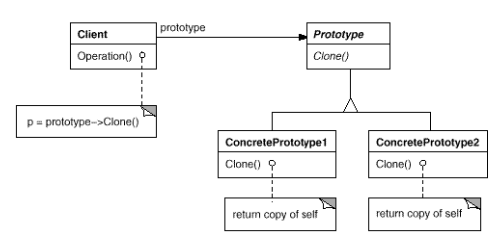
\includegraphics[width=0.6\textwidth]{img/prototype.png}
\caption{\label{fig:prototype-class-diagram}Prototype Class Diagram}
\end{figure}

\subsubsection{Singleton}
\label{sec:orgd3b9bf2}
The Singleton pattern ensures that a class has only one (global) instance.
Additionally, it provides easy access to this element.

However, you should \textbf{NOT} use it in your software.
It is basically a global variable.
Therefore, not testable and difficult to maintain.

If you want something like singleton, you should use a simple factory which always returns the same instance.


\lstset{language=java,label=lst:singelton-alternative-in-code,caption={Singelton alternative in code},captionpos=b,numbers=none}
\begin{lstlisting}
class SingletonFactory {
    private static object myInstance;

    public object createObject() {
	if (SingletonFactory.myInstance == null) {
	    SingletonFactory.myInstance = new();
	}
	return SingletonFactory.myInstance;
    }
}
\end{lstlisting}

\subsection{Structural Patterns}
\label{sec:orga3ea2e8}
\subsubsection{Adapter}
\label{sec:org11d2cd0}
The Adapter Design Pattern is used to make a class compatible to others (like a power adapter).
The adapter pattern has two different types:
\begin{itemize}
\item class adapter
\item object adapter
\end{itemize}


Both patterns do the same thing.
The class adapter inherits from the target \textbf{AND} from the adaptee (\ref{fig:class-adapter-class-diagram}).
The object adapter inherits only from the target and holds the adaptee as an instance variable (\ref{fig:object-adapter-class-diagram}).

The class adapter is not often used because many languages do not support multi-inheritance, and you should favor object composition over class inheritance.

\begin{figure}[h]
  \centering
  \begin{subfigure}{0.4\textwidth}
    \centering
    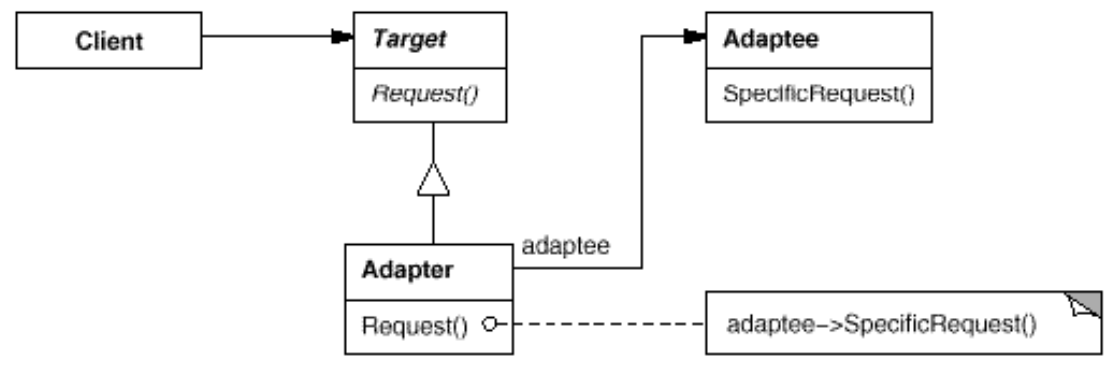
\includegraphics[width=3in]{img/object_adapter.png}
    \caption{Object Adapter Class Diagram \label{fig:object-adapter-class-diagram}}
  \end{subfigure}
  \hfill
  \begin{subfigure}{0.4\textwidth}
    \centering
    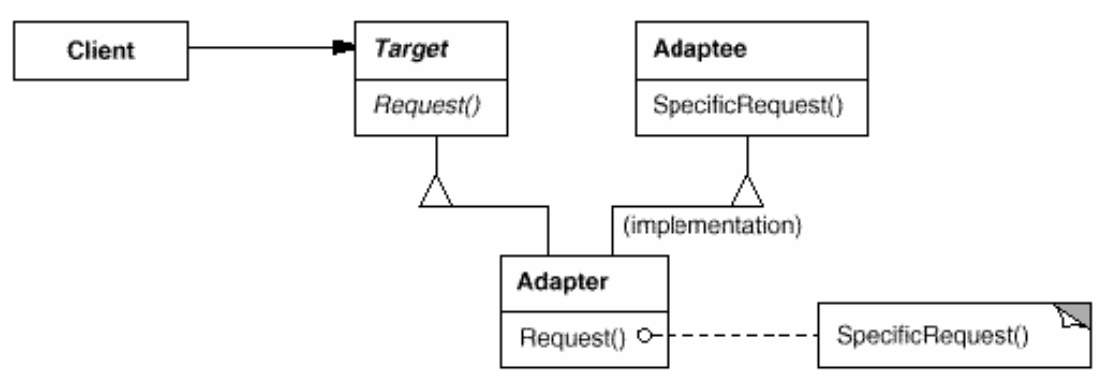
\includegraphics[width=3in]{img/class_adapter.png}
    \caption{Class Adapter Class Diagram \label{fig:class-adapter-class-diagram}}
  \end{subfigure}
  \caption{
    \label{fig:adapter-class-diagrams}
    Adapter Class Diagrams
  }
\end{figure}

\subsubsection{Bridge}
\label{sec:org015c435}
The Bridge Design Pattern is used to decouple an abstraction from its implementation so that the two can vary independently.

\begin{figure}[htbp]
\centering
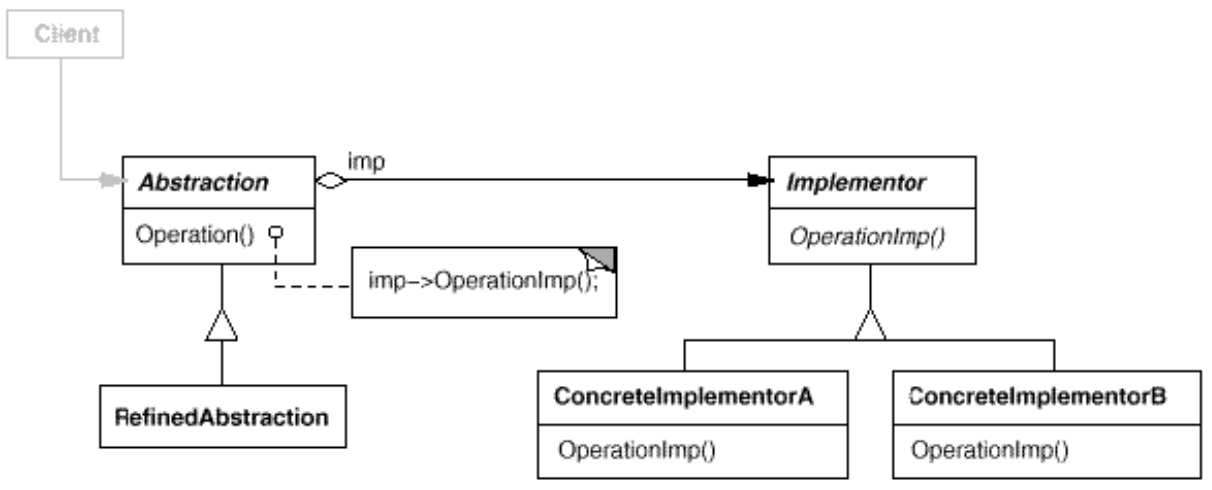
\includegraphics[width=0.6\textwidth]{img/bridge.png}
\caption{\label{fig:bridge-class-diagram}Bridge Class Diagram}
\end{figure}

\textbf{Example:}
Your application should support multiple window systems (X, Windows).
The client (your application) should be able to create windows, without committing to a concrete implementation.
Only your window implementation should depend on the target platform (X, Windows).

\subsubsection{Composite}
\label{sec:orgc3a109e}
The Composite Design Pattern is used to model a part-whole hierarchy.
The pattern let clients treat individual and compositions of objects uniformly.

\begin{center}
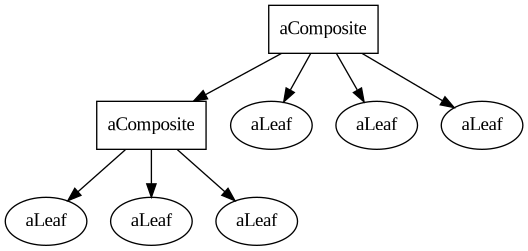
\includegraphics[width=.9\linewidth]{img/compsite_graph.png}
\end{center}


\begin{figure}[h]
  \centering
  \begin{subfigure}{0.4\textwidth}
    \centering
    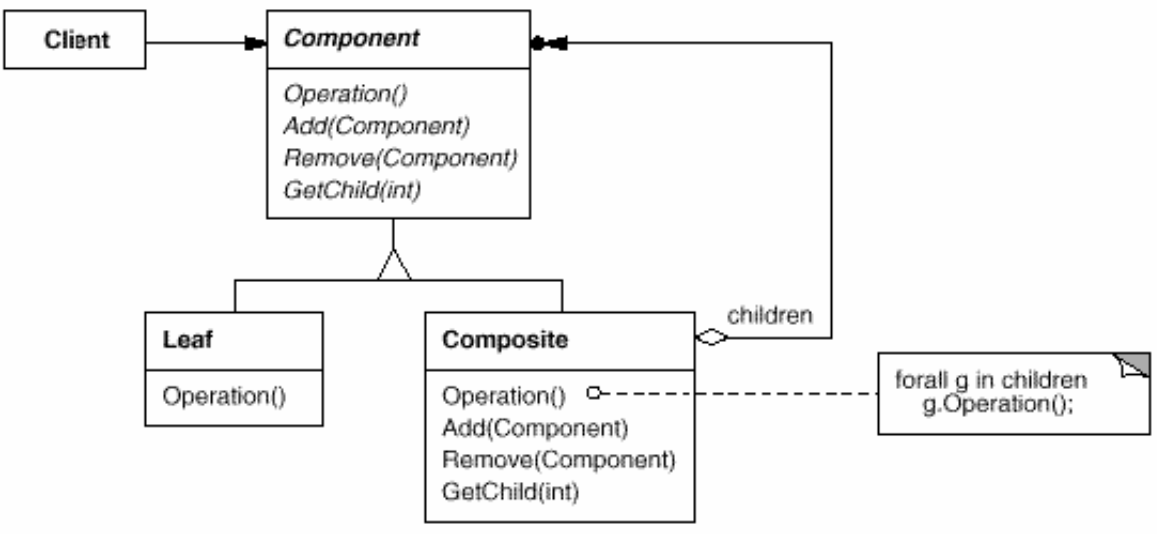
\includegraphics[width=3in]{img/composite.png}
    \caption{Composite Class Diagram \label{fig:composite-class-diagram}}
  \end{subfigure}
  \hfill
  \begin{subfigure}{0.4\textwidth}
    \centering
    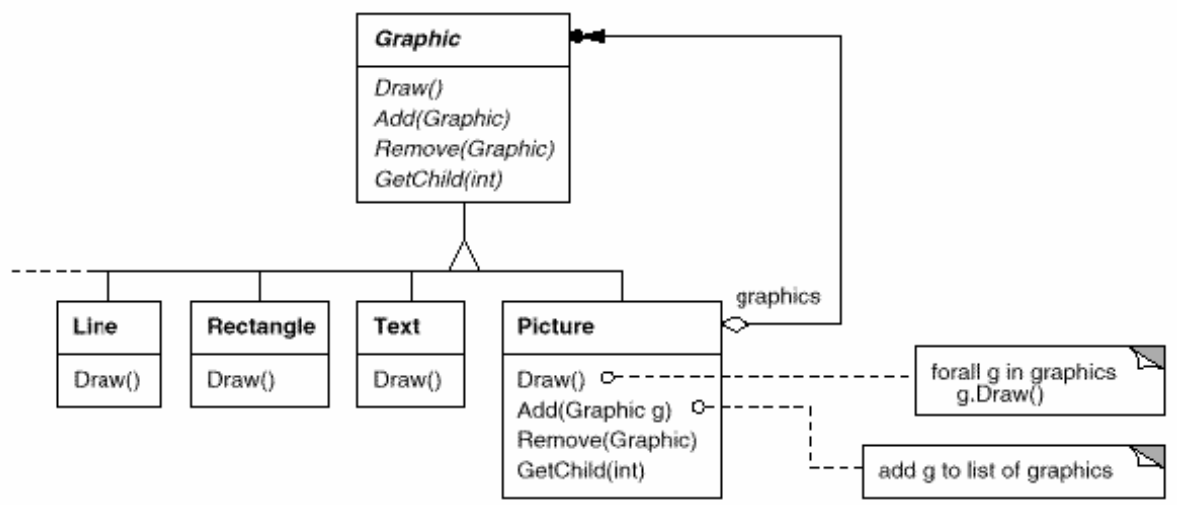
\includegraphics[width=3in]{img/example_of_composite.png}
    \caption{Example of Composite \label{fig:example-of-composite}}
  \end{subfigure}
  \caption{
    \label{fig:composite-diagrams}
    Composite Diagrams
  }
\end{figure}


\textbf{Example:}
It exists many kinds of graphics and forms (Line, Rectangle, Picture, \ldots{}).
If the client wants to draw any graphic, it does not care how draw.
Therefore, we need one function (\texttt{draw}) for all kind of graphics.
However, a picture consists of many lines, rectangles and more graphics.
This picture class has some more functions (\texttt{Add}, \texttt{Remove}, \texttt{GetChild}).
The \texttt{Draw} function iterates over all children and calls their \texttt{Draw} function.


\subsubsection{Decorator}
\label{sec:orgd705ebd}
The Decorater Pattern is used to attach additional responsibility (features) to an object dynamically.
For example, a class implements only the login mechanism.
Using the decorater pattern exception handling can be done in a separate class.


\begin{figure}[htbp]
\centering
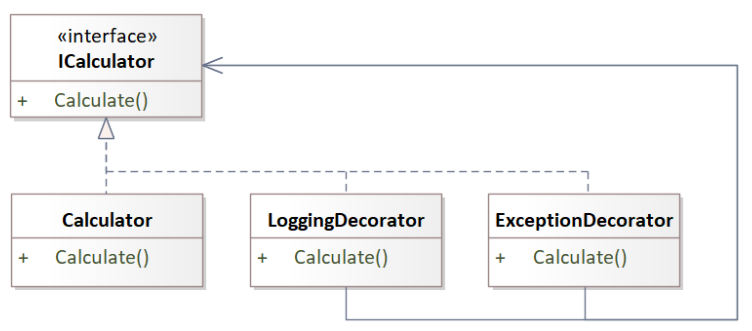
\includegraphics[width=0.6\textwidth]{img/decorater.png}
\caption{\label{fig:decrater-diagram}Decorater Diagram}
\end{figure}

\subsubsection{Facade}
\label{sec:orgb611c4a}
The Facade Design Pattern is used to provide a simple interface to a set of interfaces (subsystem).
For example the Compiler class provide an easy-to-use interface for the whole compiler subsystem (figure \ref{fig:facade-example}).


\begin{figure}[htbp]
\centering
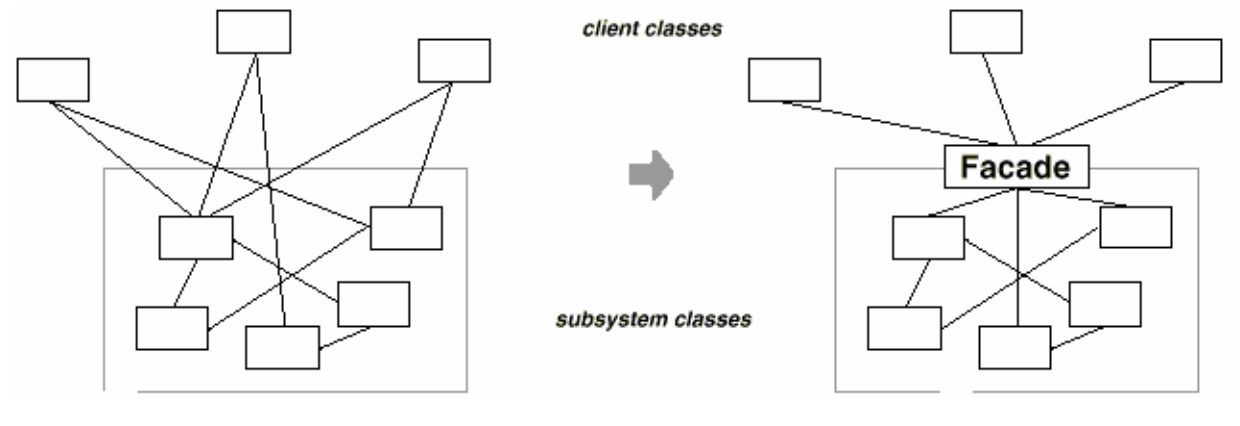
\includegraphics[width=0.6\textwidth]{img/use_case_facade.png}
\caption{\label{fig:facade-use-case}Facade Use Case}
\end{figure}


\begin{figure}[htbp]
\centering
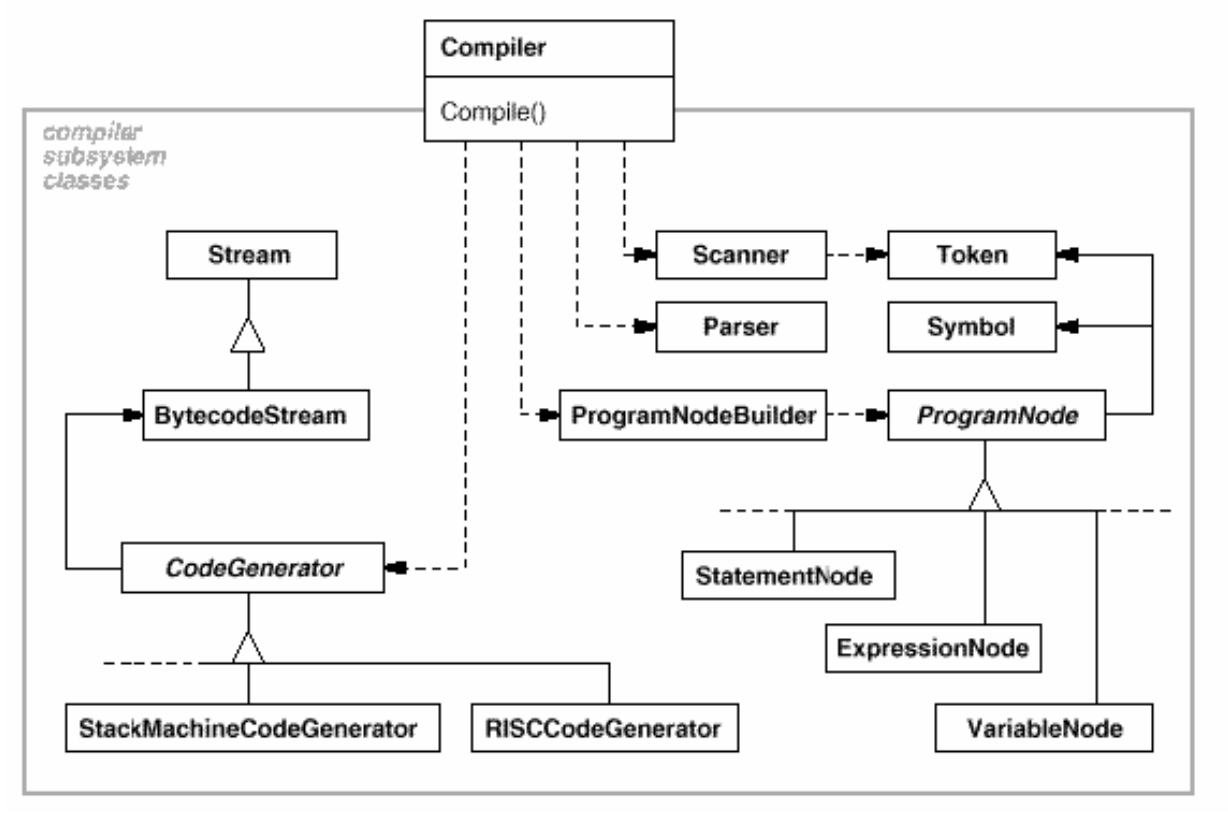
\includegraphics[width=0.6\textwidth]{img/facade_example.png}
\caption{\label{fig:facade-example}Facade Example}
\end{figure}
\subsubsection{Flyweight}
\label{sec:org1651a03}
The Flyweight pattern is used to support large number of objects efficiently.
For example, you can store every character in its own object.
In a document with 1000 characters you need more than 1000 objects.
The Flyweight pattern helps here.

In the Flyweight class is only state independent stuff stored.
Therefore, the Flyweight is shareable.
Instead, creating every time a new object with the character "a" you always reference to the same object.


\begin{figure}[htbp]
\centering
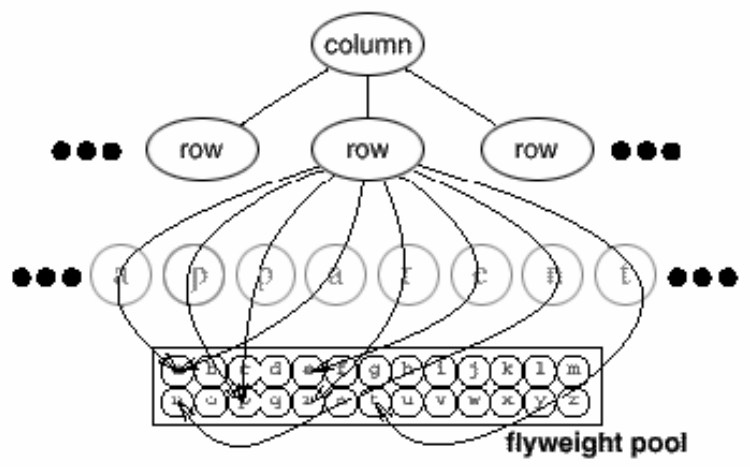
\includegraphics[width=0.6\textwidth]{img/flyweight_example.png}
\caption{\label{fig:flyweight-example}Flyweight Example}
\end{figure}


\begin{figure}[htbp]
\centering
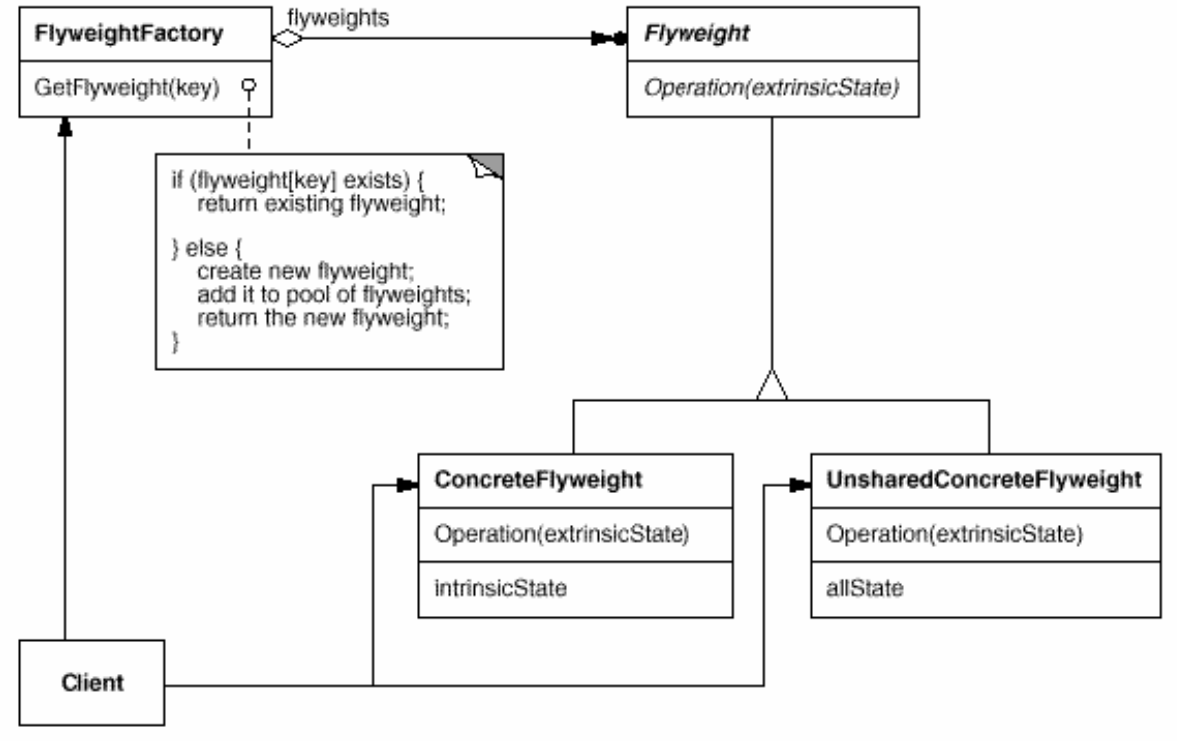
\includegraphics[width=0.6\textwidth]{img/flyweight.png}
\caption{\label{fig:flyweight-class-diagram}Flyweight Class Diagram}
\end{figure}

\subsubsection{Proxy}
\label{sec:orgacc2052}
The Proxy Design pattern provides a surrogate or placeholder for another object to control access to it.

A Feed Reader must load the news from a (slow) server.
When a frontend want to display the news before the data are available you have to provide a loading screen.
This can be easily done using the Proxy pattern.

The Proxy accepts the request, checks if the data are available.
If not, it provides the login screen.
If the news are loaded, it returns the news.


\begin{figure}[htbp]
\centering
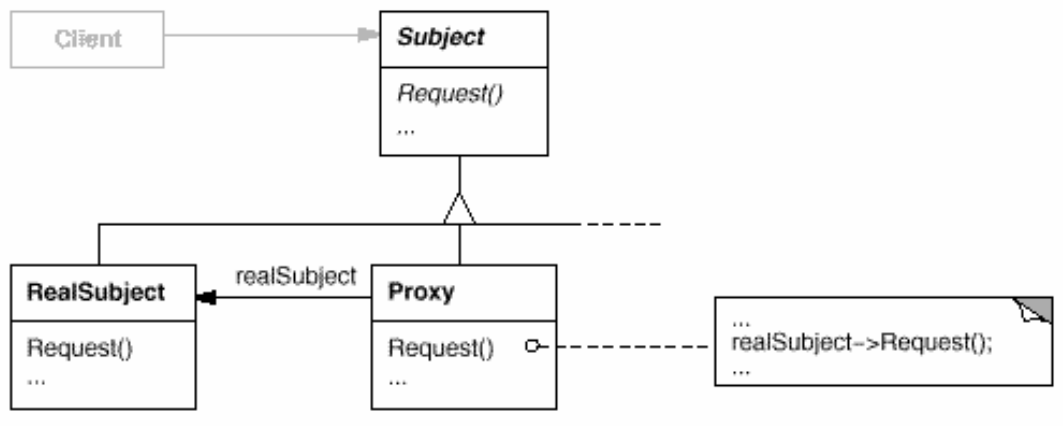
\includegraphics[width=0.6\textwidth]{img/proxy.png}
\caption{\label{fig:proxy-class-diagram}Proxy Class Diagram}
\end{figure}


\begin{figure}[htbp]
\centering
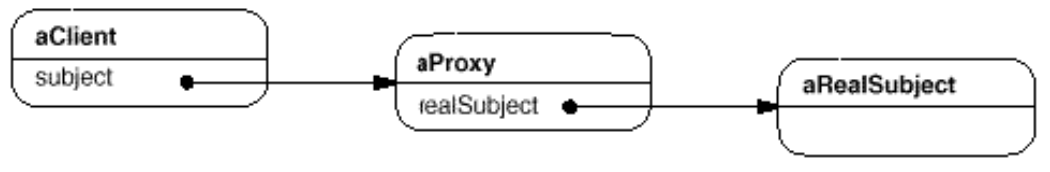
\includegraphics[width=0.6\textwidth]{img/proxy_object_diagram.png}
\caption{\label{fig:object-diagram-for-proxy}Object Diagram for proxy}
\end{figure}

\subsection{Behavioral Patterns}
\label{sec:org428e413}
\subsubsection{Chain of Responsibility}
\label{sec:org5b1d968}
The Chain of Responsibility is used to decouple the sender of a request to its receiver by giving more than one class the change to handle the request.
The first object takes the request, check if it can handle.
When yes, then handle it.
If not, forward the request to the parent / successor.


\begin{figure}[h]
  \centering
  \begin{subfigure}{0.4\textwidth}
    \centering
    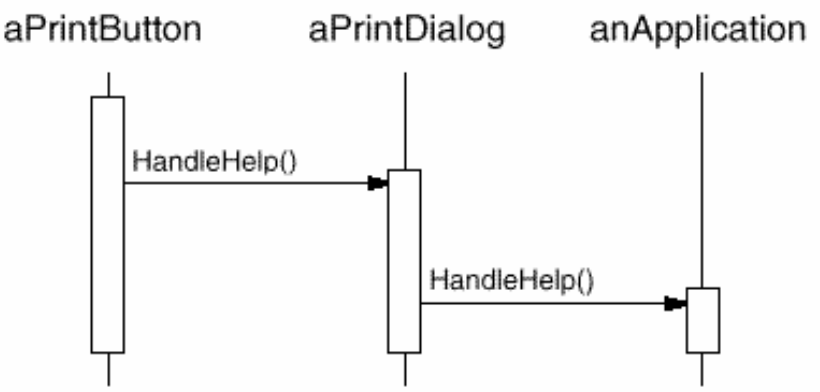
\includegraphics[width=3in]{img/chain_of_responsibility_sequence.png}
    \caption{CoR Sequence \label{fig:cor-sequence}}
  \end{subfigure}
  \hfill
  \begin{subfigure}{0.4\textwidth}
    \centering
    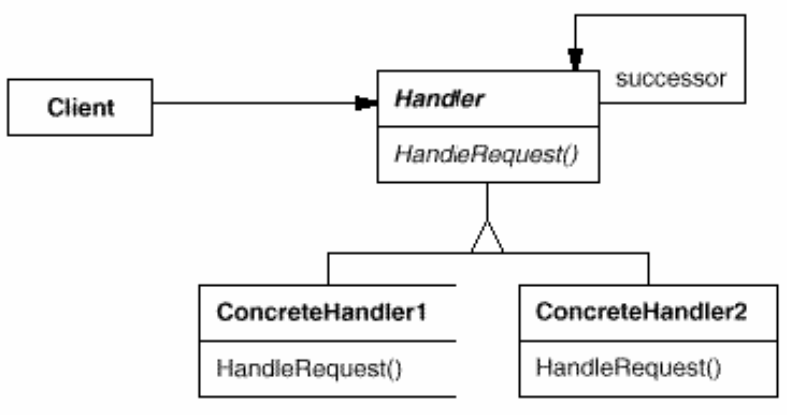
\includegraphics[width=3in]{img/chain_of_responsibility.png}
    \caption{CoR Class Diagram \label{fig:cor-class-diagram}}
  \end{subfigure}
  \caption{
    \label{fig:chain-of-responsibility-diagrams}
    Chain of Responsibilty Diagrams
  }
\end{figure}

\subsubsection{Command}
\label{sec:org2d59473}
The command pattern is used to encapsulate actions / request inside an object.
For example, the design of a framework does not know which action the button should perform.
Therefore, the button is created using a command as parameter.
As soon as the user clicks on the button, the button executions the \texttt{command.Execute()} function.

\begin{figure}[h]
  \centering
  \begin{subfigure}{0.4\textwidth}
    \centering
    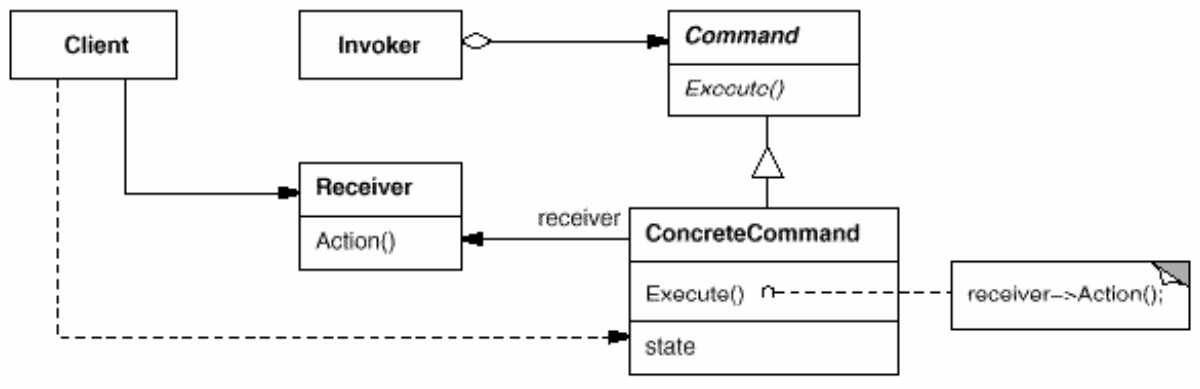
\includegraphics[width=3in]{img/command.png}
    \caption{Command Class Diagram \label{fig:command-class-diagram}}
  \end{subfigure}
  \hfill
  \begin{subfigure}{0.4\textwidth}
    \centering
    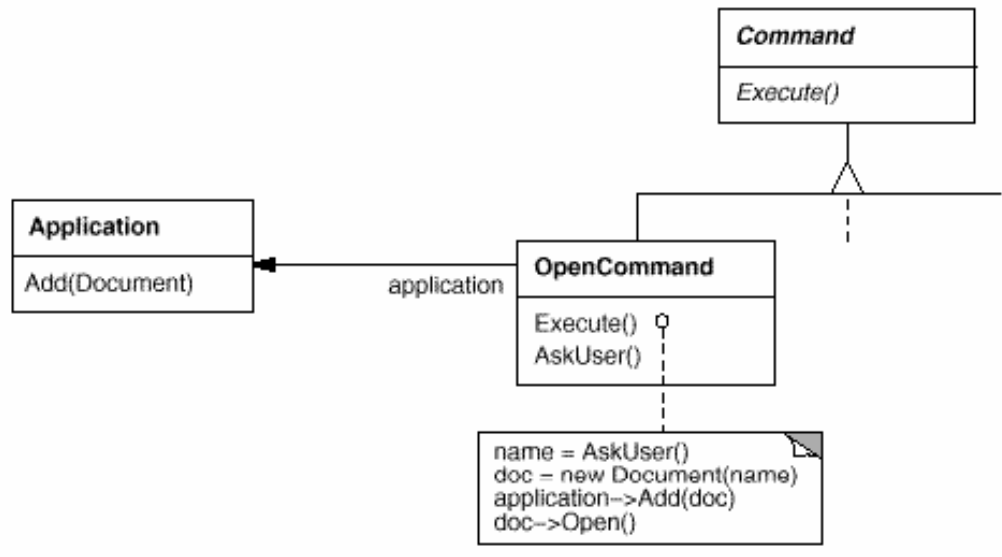
\includegraphics[width=3in]{img/example_of_command.png}
    \caption{Example of Command \label{fig:example-of-command}}
  \end{subfigure}
  \caption{
    \label{fig:command-class-diagrams}
    Command Class Diagrams
  }
\end{figure}

\subsubsection{Interpreter}
\label{sec:orge2a96f0}
The Interpreter Design Pattern is used to interpret a simple grammar / language.
Every grammar rule is modeled as one subclass.


\begin{figure}[htbp]
\centering
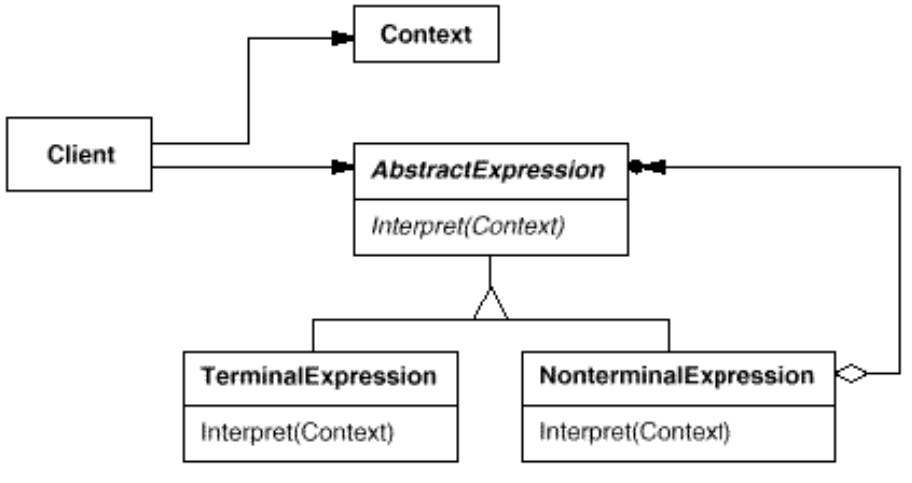
\includegraphics[width=0.6\textwidth]{img/interpreter.png}
\caption{\label{fig:interpreter-class-diagram}Interpreter Class Diagram}
\end{figure}


\textbf{My thoughts:}
Before you implement your own interpreter consider a specialized library for this.
\subsubsection{Iterator}
\label{sec:orgcac0d3a}
The iterator design pattern is used to access the items in a \href{../../../../roam/20210518131131-datastructure.org}{Data structure} (Aggregate in figure \ref{fig:iterator-class-diagram}).
The benefit of iterator is that it hides the implementation details of the data structure.

\begin{figure}[htbp]
\centering
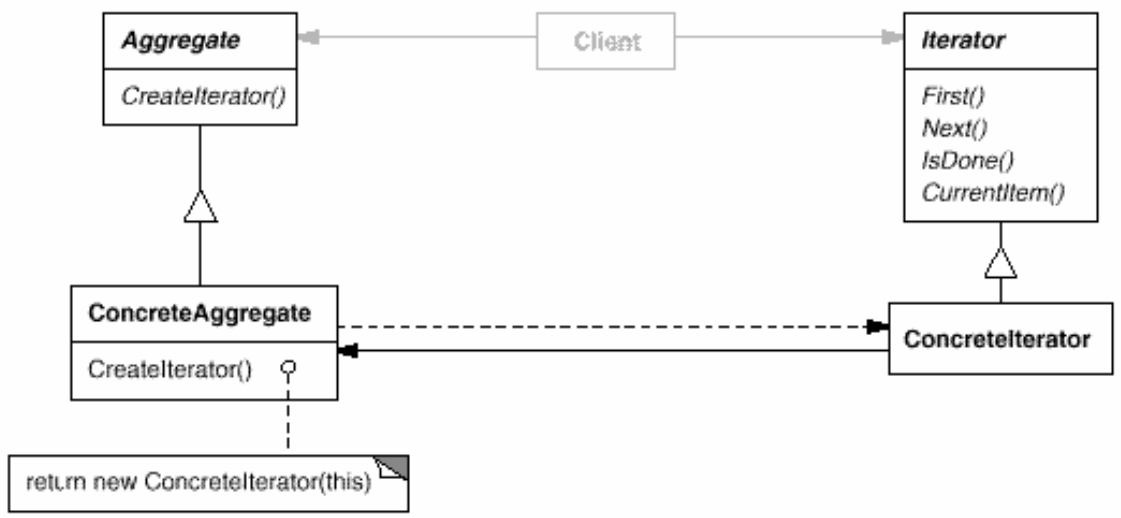
\includegraphics[width=0.6\textwidth]{img/iterator.png}
\caption{\label{fig:iterator-class-diagram}Iterator Class Diagram}
\end{figure}

\subsubsection{Mediator}
\label{sec:orga88807a}
The Mediator Design Pattern is used to encapsulate how a set of objects interact with each other.
The different objects do not have to reference each other explicit.


\begin{figure}[h]
  \centering
  \begin{subfigure}{0.4\textwidth}
    \centering
    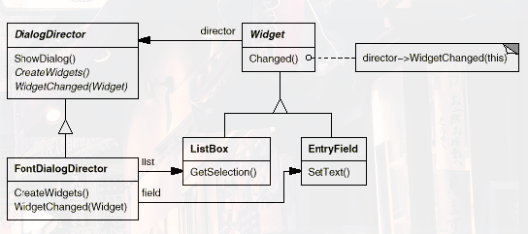
\includegraphics[width=3in]{img/mediator.png}
    \caption{Mediator Class Diagram \label{fig:mediator-class-diagram}}
  \end{subfigure}
  \hfill
  \begin{subfigure}{0.4\textwidth}
    \centering
    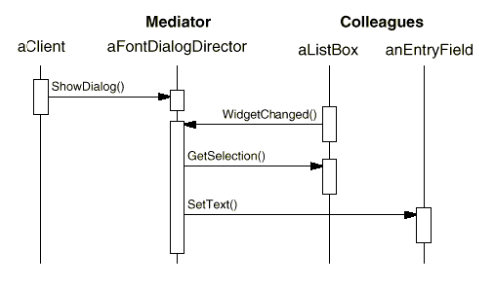
\includegraphics[width=3in]{img/mediator_sequence_diagram.png}
    \caption{Mediator Sequence Diagram \label{fig:mediator-sequence-diagram}}
  \end{subfigure}
  \caption{
    \label{fig:mp-communication-modes}
    Mediator Diagrams
  }
\end{figure}

\textbf{How does it work:}
The mediator holds a reference to every object.
The user selected some item from the list box (object A).
Object A notifies the mediator that the value has changed.
The mediator know notifies the other objects.

\subsubsection{Memento}
\label{sec:org5ee44f3}
The Memento Design Pattern is used to store an internal state.
This is often used for restoring the internal state of an object.

The object creates a memento (a copy of the state itself) and returns it to the world.
The state of the object can be restored using such a memento.
You can not change the memento and the inner live is unknown to the outer world.


\begin{figure}[htbp]
\centering
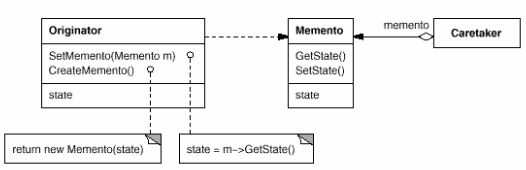
\includegraphics[width=0.6\textwidth]{img/memento.png}
\caption{\label{fig:memento-class-diagram}Memento Class Diagram}
\end{figure}

\subsubsection{Observer}
\label{sec:org5ecdc79}

The goal of the Observer Pattern is to resolve a cyclic dependency.
The Pattern consists of two objects:
\begin{itemize}
\item Subject: is monitored (e.g. a model)
\item Observer: monitors the subject (e.g. a view)
\end{itemize}


The observer register itself on the subject.
The only requirement is that the subject implements a specific interface.
Using this approach the domain does not have to need anything from the view (excepted the interface).

\begin{figure}[htbp]
\centering
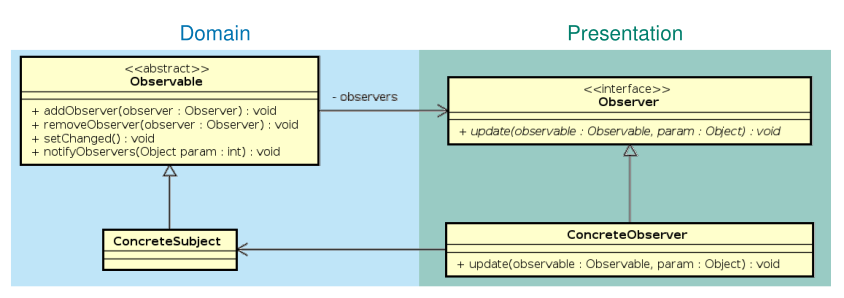
\includegraphics[width=0.6\textwidth]{img/java_observer_pattern.png}
\caption{\label{fig:observer-class-diagram}Observer Class Diagram}
\end{figure}

\subsubsection{State}
\label{sec:org3e4b033}

The state pattern is used allow an object to alter its internal behavior depending on its state.
The object will appear to change its class.

\begin{figure}[h]
  \centering
  \begin{subfigure}{0.4\textwidth}
    \centering
    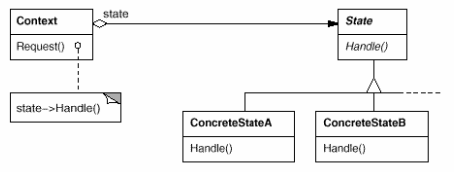
\includegraphics[width=3in]{img/state.png}
    \caption{State Class Diagram \label{fig:state-class-diagram}}
  \end{subfigure}
  \hfill
  \begin{subfigure}{0.4\textwidth}
    \centering
    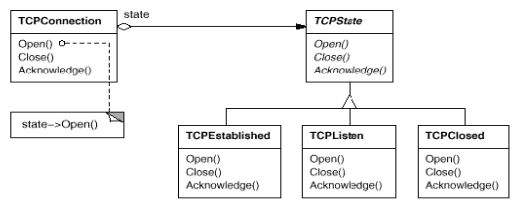
\includegraphics[width=3in]{img/state_example.png}
    \caption{TCP Connection with State \label{fig:tcp-connection-with-state}}
  \end{subfigure}
  \caption{
    \label{fig:state-class-diagrams}
    State Class Diagrams
  }
\end{figure}

\subsubsection{Strategy}
\label{sec:orge14805c}

The Strategy Pattern is used to encapsulate an algorithm in an object.
With this approach you can change the algorithm at runtime.

\begin{figure}[htbp]
\centering
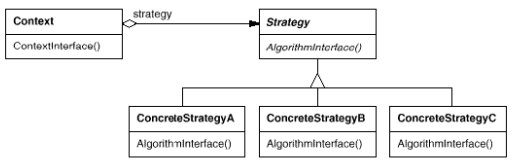
\includegraphics[width=0.6\textwidth]{img/strategy.png}
\caption{\label{fig:strategy-class-diagram}Strategy Class Diagram}
\end{figure}
\end{document}